\pentry{矢量的叉乘\upref{Cross}}

连续两个叉乘的化简也叫 BAC-CAB 定理
\begin{gather}
\vec A \cross (\vec B \cross \vec C) = \vec B \vdot (\vec A \vdot \vec C) - \vec C \vdot (\vec A \vdot \vec B)\\
(\vec B \cross \vec C) \cross \vec A = \vec C \vdot (\vec A \vdot \vec B) - \vec B \vdot (\vec A \vdot \vec C)
\end{gather}

这个定理既可以“暴力破解”,也可以用几何的方法证明.以下对几何原理略作说明,便可解释该公式的结构,方便理解和记忆.考察第一条式子,先计算 $\vec B \cross \vec C$ (命名为 $\vec D$ )方向垂直于 $\vec B$ 和 $\vec C$ 所在平面.又因为 $\vec A \cross \vec D$ 垂直于 $\vec D$, 所以结果还是落到 $\vec B$ 和 $\vec C$ 所在平面,所以等式右边是 $\vec B$ 和 $\vec C$ 的线性组合.

这里介绍一种简单的记忆方法,括号外的矢量在哪边,括号内靠近那边的矢量所在的项前面就是正号,另一项前面则是负号,如\autoref{TriCro_fig1} 所示.

\begin{figure}[ht]
\centering
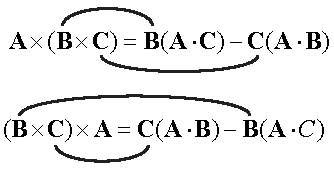
\includegraphics[width=6cm]{./figures/TriCro.pdf}
\caption{三矢量叉乘的化简}\label{TriCro_fig1}
\end{figure}
 
% 代数证明
% 多一事不如少一事!
% (使用求和符号和 epsilon 符号)
% 未完成
